\tikzset{every picture/.style={line width=0.75pt}} %set default line width to 0.75pt        
\begin{center}
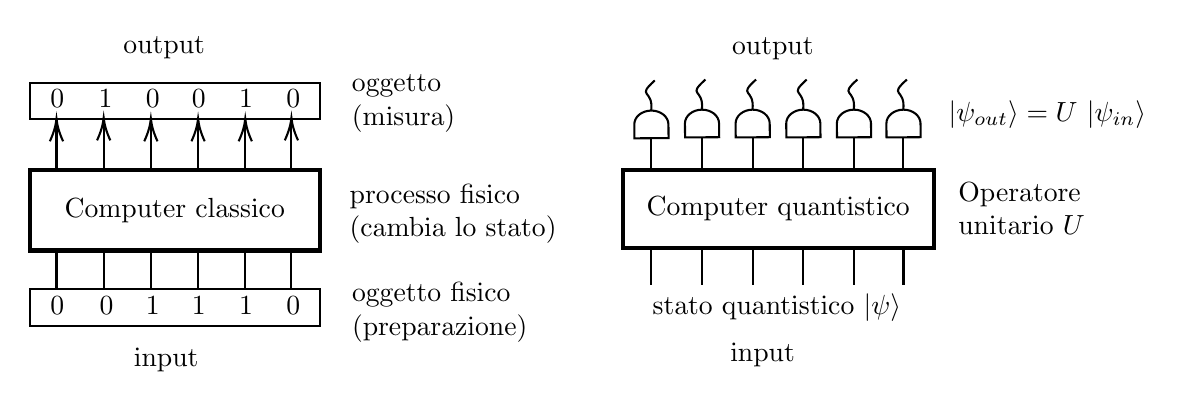
\begin{tikzpicture}[x=0.75pt,y=0.75pt,yscale=-1,xscale=0.97]
%uncomment if require: \path (0,300); %set diagram left start at 0, and has height of 300

%Shape: Rectangle [id:dp3370854768451652] 
\draw  [line width=1.5]  (38.19,137.13) -- (182.22,137.13) -- (182.22,175.83) -- (38.19,175.83) -- cycle ;
%Straight Lines [id:da444794365909732] 
\draw    (51.47,176.17) -- (51.47,194.51) ;


%Straight Lines [id:da3309151478008787] 
\draw    (74.91,175.83) -- (74.91,194.17) ;


%Straight Lines [id:da5291423146743008] 
\draw    (98.35,176.17) -- (98.35,194.51) ;


%Straight Lines [id:da8471848239987096] 
\draw    (121.8,176.17) -- (121.8,194.51) ;


%Straight Lines [id:da5685433525068389] 
\draw    (145.24,176.17) -- (145.24,194.51) ;


%Straight Lines [id:da37769970174090206] 
\draw    (168.16,175.83) -- (168.16,194.17) ;


%Straight Lines [id:da3063143558848054] 
\draw    (51.47,114.31) -- (51.47,136.9) ;

\draw [shift={(51.47,112.31)}, rotate = 90] [color={rgb, 255:red, 0; green, 0; blue, 0 }  ][line width=0.75]    (10.93,-3.29) .. controls (6.95,-1.4) and (3.31,-0.3) .. (0,0) .. controls (3.31,0.3) and (6.95,1.4) .. (10.93,3.29)   ;
%Straight Lines [id:da7551493211306404] 
\draw    (74.91,113.85) -- (74.91,136.44) ;

\draw [shift={(74.91,111.85)}, rotate = 90] [color={rgb, 255:red, 0; green, 0; blue, 0 }  ][line width=0.75]    (10.93,-3.29) .. controls (6.95,-1.4) and (3.31,-0.3) .. (0,0) .. controls (3.31,0.3) and (6.95,1.4) .. (10.93,3.29)   ;
%Straight Lines [id:da8373218927741573] 
\draw    (98.35,114.31) -- (98.35,136.9) ;

\draw [shift={(98.35,112.31)}, rotate = 90] [color={rgb, 255:red, 0; green, 0; blue, 0 }  ][line width=0.75]    (10.93,-3.29) .. controls (6.95,-1.4) and (3.31,-0.3) .. (0,0) .. controls (3.31,0.3) and (6.95,1.4) .. (10.93,3.29)   ;
%Straight Lines [id:da8820817105984171] 
\draw    (121.8,114.31) -- (121.8,136.9) ;

\draw [shift={(121.8,112.31)}, rotate = 90] [color={rgb, 255:red, 0; green, 0; blue, 0 }  ][line width=0.75]    (10.93,-3.29) .. controls (6.95,-1.4) and (3.31,-0.3) .. (0,0) .. controls (3.31,0.3) and (6.95,1.4) .. (10.93,3.29)   ;
%Straight Lines [id:da23173642990564458] 
\draw    (145.24,114.31) -- (145.24,136.9) ;

\draw [shift={(145.24,112.31)}, rotate = 90] [color={rgb, 255:red, 0; green, 0; blue, 0 }  ][line width=0.75]    (10.93,-3.29) .. controls (6.95,-1.4) and (3.31,-0.3) .. (0,0) .. controls (3.31,0.3) and (6.95,1.4) .. (10.93,3.29)   ;
%Straight Lines [id:da3352885240092238] 
\draw    (168.16,113.85) -- (168.16,136.44) ;

\draw [shift={(168.16,111.85)}, rotate = 90] [color={rgb, 255:red, 0; green, 0; blue, 0 }  ][line width=0.75]    (10.93,-3.29) .. controls (6.95,-1.4) and (3.31,-0.3) .. (0,0) .. controls (3.31,0.3) and (6.95,1.4) .. (10.93,3.29)   ;
%Shape: Rectangle [id:dp8501179019878584] 
\draw   (38.19,95) -- (182.22,95) -- (182.22,112.53) -- (38.19,112.53) -- cycle ;
%Shape: Rectangle [id:dp18502125567242067] 
\draw   (38.19,194.51) -- (182.22,194.51) -- (182.22,212.04) -- (38.19,212.04) -- cycle ;
%Shape: Rectangle [id:dp08080369161895873] 
\draw  [line width=1.5]  (332.7,137.23) -- (487.26,137.23) -- (487.26,174.6) -- (332.7,174.6) -- cycle ;
%Straight Lines [id:da5174976099608133] 
\draw    (346.96,174.93) -- (346.96,192.62) ;


%Straight Lines [id:da3906594571053619] 
\draw    (372.11,174.6) -- (372.11,192.29) ;


%Straight Lines [id:da08487629323958013] 
\draw    (397.27,174.93) -- (397.27,192.62) ;


%Straight Lines [id:da6583582327013684] 
\draw    (422.42,174.93) -- (422.42,192.62) ;


%Straight Lines [id:da8933659412949497] 
\draw    (447.57,174.93) -- (447.57,192.62) ;


%Straight Lines [id:da03377065386226974] 
\draw    (472.17,174.6) -- (472.17,192.29) ;


%Straight Lines [id:da7845188854936893] 
\draw    (346.96,121.69) -- (346.96,137.01) ;


%Straight Lines [id:da5758058639542603] 
\draw    (372.11,121.4) -- (372.11,136.73) ;


%Straight Lines [id:da8825945599217435] 
\draw    (397.27,121.69) -- (397.27,137.01) ;


%Straight Lines [id:da027631106900613434] 
\draw    (422.42,121.69) -- (422.42,137.01) ;


%Straight Lines [id:da9616245238371959] 
\draw    (447.57,121.69) -- (447.57,137.01) ;


%Straight Lines [id:da6887376007663764] 
\draw    (471.89,121.69) -- (471.89,137.01) ;


%Flowchart: Delay [id:dp748952144669494] 
\draw   (338.54,121.81) -- (338.47,115.15) .. controls (338.43,111.48) and (342.19,108.47) .. (346.87,108.44) .. controls (351.55,108.41) and (355.38,111.37) .. (355.42,115.04) -- (355.49,121.7) -- cycle ;
%Flowchart: Delay [id:dp3966652317655148] 
\draw   (363.69,121.37) -- (363.62,114.71) .. controls (363.58,111.04) and (367.35,108.03) .. (372.03,108) .. controls (376.71,107.97) and (380.53,110.93) .. (380.57,114.61) -- (380.64,121.27) -- cycle ;
%Flowchart: Delay [id:dp8688199158082022] 
\draw   (388.85,121.37) -- (388.78,114.71) .. controls (388.74,111.04) and (392.5,108.03) .. (397.18,108) .. controls (401.86,107.97) and (405.69,110.93) .. (405.72,114.61) -- (405.8,121.27) -- cycle ;
%Flowchart: Delay [id:dp8086320640430136] 
\draw   (414,121.37) -- (413.93,114.71) .. controls (413.89,111.04) and (417.65,108.03) .. (422.33,108) .. controls (427.01,107.97) and (430.84,110.93) .. (430.88,114.61) -- (430.95,121.27) -- cycle ;
%Flowchart: Delay [id:dp722358729241092] 
\draw   (439.16,121.37) -- (439.08,114.71) .. controls (439.05,111.04) and (442.81,108.03) .. (447.49,108) .. controls (452.17,107.97) and (455.99,110.93) .. (456.03,114.61) -- (456.1,121.27) -- cycle ;
%Flowchart: Delay [id:dp16472187429517238] 
\draw   (463.75,121.37) -- (463.68,114.71) .. controls (463.64,111.04) and (467.4,108.03) .. (472.08,108) .. controls (476.76,107.97) and (480.59,110.93) .. (480.63,114.61) -- (480.7,121.27) -- cycle ;
%Curve Lines [id:da02121963440081065] 
\draw    (373.79,93.49) .. controls (364.29,101.84) and (373.23,97.44) .. (372.03,108) ;


%Curve Lines [id:da31983882752062054] 
\draw    (348.64,93.93) .. controls (339.13,102.28) and (348.08,97.88) .. (346.87,108.44) ;


%Curve Lines [id:da4623293987746533] 
\draw    (398.94,93.49) .. controls (389.44,101.84) and (398.38,97.44) .. (397.18,108) ;


%Curve Lines [id:da5783366480443313] 
\draw    (424.1,93.49) .. controls (414.59,101.84) and (423.54,97.44) .. (422.33,108) ;


%Curve Lines [id:da4188892016494363] 
\draw    (449.25,93.49) .. controls (439.75,101.84) and (448.69,97.44) .. (447.49,108) ;


%Curve Lines [id:da14876622747392365] 
\draw    (473.84,93.49) .. controls (464.34,101.84) and (473.28,97.44) .. (472.08,108) ;



% Text Node
\draw (110.2,156.48) node  [align=left] {Computer classico};
% Text Node
\draw (51.86,102.86) node   {$0$};
% Text Node
\draw (75.82,102.86) node   {$1$};
% Text Node
\draw (99.27,102.86) node   {$0$};
% Text Node
\draw (122.19,102.86) node   {$0$};
% Text Node
\draw (145.63,102.86) node   {$1$};
% Text Node
\draw (169.07,102.86) node   {$0$};
% Text Node
\draw (51.86,202.36) node   {$0$};
% Text Node
\draw (76.34,202.36) node   {$0$};
% Text Node
\draw (99.27,202.36) node   {$1$};
% Text Node
\draw (122.19,202.36) node   {$1$};
% Text Node
\draw (145.63,202.36) node   {$1$};
% Text Node
\draw (169.07,202.36) node   {$0$};
% Text Node
\draw (105.93,228.61) node  [align=left] {input};
% Text Node
\draw (104.97,78.34) node  [align=left] {output};
% Text Node
\draw (241.82,205.7) node  [align=left] {oggetto fisico\\(preparazione)};
% Text Node
\draw (248.47,158.25) node  [align=left] {processo fisico\\(cambia lo stato)};
% Text Node
\draw (223.87,104.97) node  [align=left] {oggetto\\(misura)};
% Text Node
\draw (409.98,155.91) node  [align=left] {Computer quantistico};
% Text Node
\draw (402.17,226.25) node  [align=left] {input};
% Text Node
\draw (407.28,78.58) node  [align=left] {output};
% Text Node
\draw (409.28,203.17) node  [align=left] {stato quantistico $\displaystyle |\psi \rangle $};
% Text Node
\draw (530.86,155.69) node  [align=left] {Operatore\\unitario $\displaystyle U$};
% Text Node
\draw (532.54,110.19) node  [align=left] {$ $};
% Text Node
\draw (545.95,110.19) node   {$|\psi _{out} \rangle =U\ |\psi _{in} \rangle \ $};


\end{tikzpicture}
\end{center}